\documentclass{article}
\usepackage{amsmath, amssymb}
\usepackage{mathptmx}
\usepackage{parskip}
\usepackage{makecell}
\usepackage{stix}
\usepackage{geometry}
\usepackage{booktabs,tabularx}
\usepackage{bm}
\usepackage{graphicx}

\geometry{legalpaper, margin=1in}

\title{Probability Distributions}
\date{April, 2023}
\author{Suneet Tipirneni}

\begin{document}
\maketitle

\section{The Covariance Matrix}

In the univariate normal distribution the covariance is the represented as $\sigma^2$, in the case of the multivariate we use $\Sigma$ to represent the covariance matrix.  \par

\begin{equation}\label{eq:norm}
	Pr\left( x,y \right) = \frac{1}{\left( 2\pi \right)^{\frac{D}{2}}\sqrt{ \mid \Sigma \mid}}\exp\left[ -0.5\left( \pmb{x} - \pmb{\mu} \right)^{T} \pmb{\Sigma}^{-1} \left( \pmb{x} - \pmb{\mu} \right)  \right] 
\end{equation}

\section{Type of Covariance Matrices}

There are three forms of covariance matrices, spherical, diagonal, and full:

\begin{align}
	\pmb{\Sigma}_{sphere} = \begin{bmatrix} \sigma^2 & 0 \\ 0 & \sigma^2  \end{bmatrix} &&
	\pmb{\Sigma}_{diag} = \begin{bmatrix} \sigma_1^2 & 0 \\ 0 & \sigma_2^2 \end{bmatrix} && 
	\pmb{\Sigma}_{full} = \begin{bmatrix} \sigma_{11}^2 & \sigma_{12}^2 \\ \sigma_{21}^2 & \sigma_{22}^2 \end{bmatrix} 
\end{align}

Where $D$ is the number of dimensions.

\begin{figure}[htpb]
	\centering
	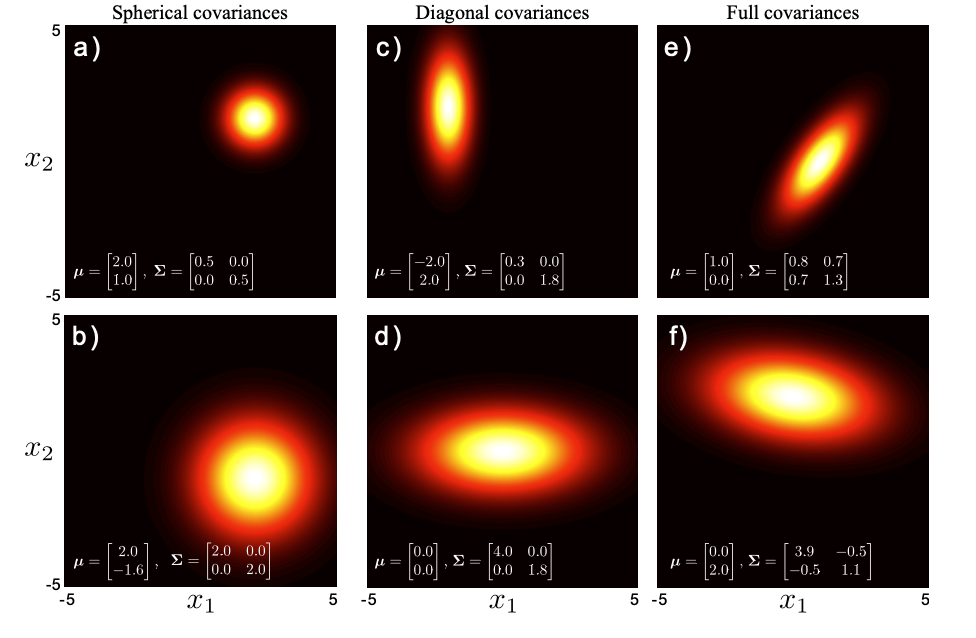
\includegraphics[width=0.8\textwidth]{imgs/type-cov.png}
	\caption{The different kinds of covariance matrices represented visually provided by \cite{princeCVMLI2012}}
	\label{fig:type-cov}
\end{figure}

\subsubsection{Spherical and Diagonal independence}

When the convariance matrix is spherical or diagonal both variables are independent. We can prove it for the bivariate diagonal case where $D=2$ by the following equivalence:

\begin{align*}
	Pr\left( x_1,x_2 \right) &= \frac{1}{2\pi \sqrt{\mid \Sigma  \mid} } \exp\left[ -\frac{1}{2} \begin{pmatrix} x_1 & x_2 \end{pmatrix} \Sigma^{-1} \begin{pmatrix} x_1 \\ x_2  \end{pmatrix}     \right]  \\
							 &= \frac{1}{2\pi \sigma_1 \sigma_2} \exp\left[ -\frac{1}{2} \begin{pmatrix} x_1 & x_2 \end{pmatrix} \begin{pmatrix} \sigma_1^{-2} & 0 \\ 0 & \sigma_2^{-2} \end{pmatrix} \begin{pmatrix} x_1 \\ x_2 \end{pmatrix}     \right] \\
						 &= \frac{1}{2\pi \sigma_1 \sigma_2 } \exp\left[ -\frac{x_1^2}{2\sigma_1^2} - \frac{x_2^2}{2\sigma^2_2} \right] \\
						 &= \frac{1}{\sqrt{2\pi \sigma^2_1}} \exp\left[ -\frac{x_1^2}{2\sigma_1^2}  \right] \frac{1}{\sqrt{2\pi \sigma^2_2}} \exp\left[ -\frac{x_2^2}{2\sigma_2^2}  \right] \\
						 &= Pr\left( x_1 \right) Pr\left( x_2 \right) 
\end{align*}

\section{Decomposition of covariance}

A full covariance matrix can be decomposed into a diagonal matrix multiplied by rotation matricies. 

\begin{figure}[htpb]
	\centering
	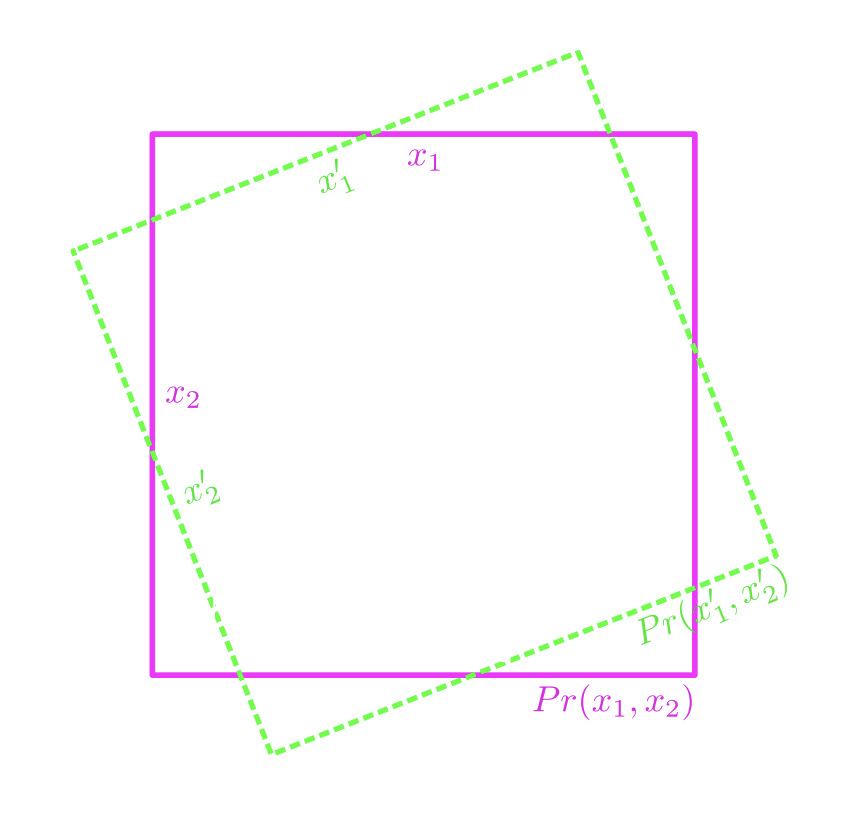
\includegraphics[width=0.5\textwidth]{imgs/full-decomp.png}
	\caption{By rotating the axis of where the full convariance matrix is located we can align it to be a diagonal matrix. \cite{princeCVMLI2012}}
	\label{fig:full-decomp}
\end{figure}

As shown in figure \ref{fig:full-decomp}, we change the axis to align with the shape of the full covariance matrix. As a result of this we need to adjust our equation to account for this transformation.

We call the new covariance matrix $\Sigma^{'}_{diag}$, which is the decomposed diagonal convariance matrix. The data vector for the matrix is represented as $\pmb{x}^{'} = \left[ x_1^{'},x_2^{'} \right]^{T} $ where $\pmb{x^{'}}$ is calculated from $\pmb{x^{'}} \pmb{R}\pmb{x}$. The probability distribution is:

\begin{align*}
	Pr\left( \pmb{x^{'}} \right) = \frac{1}{\left( 2\pi \right)^{\frac{D}{2}}  \mid \Sigma^{'}_{diag}  \mid^{\frac{1}{2}} } \exp \left[ -0.5\pmb{x}^{'T} \Sigma_{diag}^{'-1} \pmb{x^{'}} \right]
\end{align*}

To convert back to the original we substitute $\pmb{x'}$ with $\pmb{Rx}$:

\begin{align*}
	Pr\left( \pmb{x} \right) &= \frac{1}{\left( 2\pi \right)^{\frac{D}{2}} \mid \Sigma_{diag}^{'} \mid^{\frac{1}{2}} } \exp{\left[ -0.5 (\pmb{Rx})^{T} \Sigma_{diag}^{'-1} \pmb{Rx} \right]  } \\
							 &= \frac{1}{\left( 2\pi \right)^{\frac{D}{2}} \mid \pmb{R}^{T} \Sigma_{diag}^{'} \pmb{R} \mid^{\frac{1}{2}} } \exp{\left[ -0.5 \pmb{x}^{T} (\pmb{R}^{T} \Sigma_{diag} \pmb{R})^{-1} \pmb{x} \right]  }
\end{align*}

The equivalence $\mid \pmb{R}^{T} \Sigma^{'} \pmb{R} \mid = \mid \pmb{R}^{T}  \mid \cdot \mid \Sigma^{'}  \mid \cdot \mid \pmb{R} \mid = 1 \cdot \mid \Sigma^{'} \mid \cdot 1 = \mid \Sigma^{'} \mid$. Recall the determinant of a rotation matrix is always 1.



\bibliographystyle{plain}
\bibliography{refs}

\end{document}
